% !TeX program = LuaLaTeX
\documentclass[aspectratio=169, 10pt]{beamer}\usepackage[]{graphicx}\usepackage[]{xcolor}
% maxwidth is the original width if it is less than linewidth
% otherwise use linewidth (to make sure the graphics do not exceed the margin)
\makeatletter
\def\maxwidth{ %
  \ifdim\Gin@nat@width>\linewidth
    \linewidth
  \else
    \Gin@nat@width
  \fi
}
\makeatother

\definecolor{fgcolor}{rgb}{0.345, 0.345, 0.345}
\newcommand{\hlnum}[1]{\textcolor[rgb]{0.686,0.059,0.569}{#1}}%
\newcommand{\hlsng}[1]{\textcolor[rgb]{0.192,0.494,0.8}{#1}}%
\newcommand{\hlcom}[1]{\textcolor[rgb]{0.678,0.584,0.686}{\textit{#1}}}%
\newcommand{\hlopt}[1]{\textcolor[rgb]{0,0,0}{#1}}%
\newcommand{\hldef}[1]{\textcolor[rgb]{0.345,0.345,0.345}{#1}}%
\newcommand{\hlkwa}[1]{\textcolor[rgb]{0.161,0.373,0.58}{\textbf{#1}}}%
\newcommand{\hlkwb}[1]{\textcolor[rgb]{0.69,0.353,0.396}{#1}}%
\newcommand{\hlkwc}[1]{\textcolor[rgb]{0.333,0.667,0.333}{#1}}%
\newcommand{\hlkwd}[1]{\textcolor[rgb]{0.737,0.353,0.396}{\textbf{#1}}}%
\let\hlipl\hlkwb

\usepackage{framed}
\makeatletter
\newenvironment{kframe}{%
 \def\at@end@of@kframe{}%
 \ifinner\ifhmode%
  \def\at@end@of@kframe{\end{minipage}}%
  \begin{minipage}{\columnwidth}%
 \fi\fi%
 \def\FrameCommand##1{\hskip\@totalleftmargin \hskip-\fboxsep
 \colorbox{shadecolor}{##1}\hskip-\fboxsep
     % There is no \\@totalrightmargin, so:
     \hskip-\linewidth \hskip-\@totalleftmargin \hskip\columnwidth}%
 \MakeFramed {\advance\hsize-\width
   \@totalleftmargin\z@ \linewidth\hsize
   \@setminipage}}%
 {\par\unskip\endMakeFramed%
 \at@end@of@kframe}
\makeatother

\definecolor{shadecolor}{rgb}{.97, .97, .97}
\definecolor{messagecolor}{rgb}{0, 0, 0}
\definecolor{warningcolor}{rgb}{1, 0, 1}
\definecolor{errorcolor}{rgb}{1, 0, 0}
\newenvironment{knitrout}{}{} % an empty environment to be redefined in TeX

\usepackage{alltt}
\usetheme{gotham}

	\gothamset{
		numbering=totalframenumber,
		% tocframe template= gotham simple,
		tocframe template= gotham bullet,
		% progressbar position=circlehead,
		progressbar position=foot,
		progressbar style=rectangle,
		progressbar mfn=on,
		parttocframe default=off,
		sectiontocframe default=off,
		subsectiontocframe default=off,
	}

	\usepackage{standalone}
	\usepackage{tikz}
	\usepackage{pgfplots}
	\usepackage{tabularray} % Typeset tabulars and arrays (contains equivalent of longtable, booktabs and dcolumn at least) 
		\UseTblrLibrary{booktabs} % to load extra commands from booktabs
	\usepackage{changepage}
	\usepackage{appendixnumberbeamer}
		\newcommand{\famName}[1]{\textsc{#1}}
	\usepackage{minted}
		\definecolor{codeback}{rgb}{0.90,0.91,0.92}
		\definecolor{codebackdark}{rgb}{0.10,0.11,0.12}
		\usemintedstyle{emacs}
		\setmintedinline[tex]{bgcolor=codeback}
		\setminted[tex]{
			autogobble,
			bgcolor=codeback,
			tabsize=4,
			extrakeywords={usetheme,institute,maketitle,subtitle,gothamset,colorlet,setbeamercolor,plain,defbeamertemplate}
		}

	\usepackage[scale=2]{ccicons}
	% \usepackage{pgfplots}
		\usepgfplotslibrary{dateplot}

	\newcommand{\themename}{\textbf{\textsc{Gotham}}}


\title[]{Innovations in Likelihood-Based Inference for State Space Models}
\subtitle{Oral Defense}
\date[]{\today}
\author[Wheeler]{Jesse Wheeler}
\institute{Department of Statistics, University of Michigan}
\titlegraphic{\hfill
\includegraphics[height=1.5cm]{gotham-logo.pdf}}
\IfFileExists{upquote.sty}{\usepackage{upquote}}{}
\begin{document}

\maketitle

	\begin{frame}[toc]{Table of contents}%
		\tableofcontents%[hideallsubsections]
	\end{frame}

	
%%%%%%%%%%%%%%%%%%%%
%%%  MAINMATTER  %%%
%%%%%%%%%%%%%%%%%%%%
% \documentclass[aspectratio=169]{beamer}

	\usepackage{standalone}
	\usepackage{tikz}
	\usepackage{pgfplots}

	\usepackage{tabularray} % Typeset tabulars and arrays (contains equivalent of longtable, booktabs and dcolumn at least) 
		\UseTblrLibrary{booktabs} % to load extra commands from booktabs

	\usepackage{natbib}
\begin{filecontents*}[overwrite]{pres.bib}
@article{Knuth92,
	author = "D.E. Knuth",
	title = "Two notes on notation",
	journal = "Amer. Math. Monthly",
	volume = "99",
	year = "1992",
	pages = "403--422",
}

@book{ConcreteMath,
	author = "R.L. Graham and D.E. Knuth and O. Patashnik",
	title = "Concrete mathematics",
	publisher = "Addison-Wesley",
	address = "Reading, MA",
	year = "1989"
}

@unpublished{Simpson,
	author = "H. Simpson",
	title = "Proof of the {R}iemann {H}ypothesis",
	note = "preprint (2003), available at \texttt{http://www.math.drofnats.edu/riemann.ps}",
	year = "2003"
}

@incollection{Er01,
	author = "P. Erd{\H o}s",
	title = "A selection of problems and results in combinatorics",
	booktitle = "Recent trends in combinatorics (Matrahaza, 1995)",
	publisher = "Cambridge Univ. Press",
	address = "Cambridge",
	pages = "1--6",
	year = "1995"
}

@article{greenwade93,
	author  = "George D. Greenwade",
	title   = "The {C}omprehensive {T}ex {A}rchive {N}etwork ({CTAN})",
	year    = "1993",
	journal = "TUGBoat",
	volume  = "14",
	number  = "3",
	pages   = "342--351"
}
\end{filecontents*}


\begin{document}

\section{Introduction: Beamer}

	% FRAME
	\begin{frame}[fragile]{Title page}
		The Title page is printed using the command:			
		\begin{verbatim}    \maketitle\end{verbatim}
		
		The element printed on this page are defined in the preamble by
		\begin{verbatim}
			\title[]{Gotham}
			\subtitle{A Modern, versatile and extendable theme for Beamer}
			\date[]{\today}
			\author[]{Romain NOËL}
			\institute{Center for modern beamer themes}
			% \titlegraphic{\hfill\includegraphics[height=1.5cm, draft]{Title_logo.pdf}}
		\end{verbatim}
	\end{frame}
	
	% FRAME
	\begin{frame}[fragile]{Plain Slide}
		The usual page is printed and defined using the command:			
		\begin{verbatim}
			\begin{frame}{Title on top of the frame}
				contenu...
			\end{frame }
		\end{verbatim}
		
		Note that the logo printed on this page are defined in the preamble by
		% \begin{verbatim}
		% 	% \logo{\includegraphics[height=1.5cm, draft]{logo.pdf}}
		% \end{verbatim}
	\end{frame}

	% FRAME
	\begin{frame}[fragile]{Sections}
		Sections group slides of the same topic
		
		\begin{verbatim}    \section{Elements}\end{verbatim}
	\end{frame}

	% FRAME
	\begin{frame}[fragile]{Typography}
		\begin{verbatim}
			The theme provides sensible defaults to
			\emph{emphasize} text, \alert{accent} parts
			or show \textbf{bold} results.
		\end{verbatim}
		
		\begin{center}becomes\end{center}
		
		The theme provides sensible defaults to \emph{emphasize} text,
		\alert{accent} parts or show \textbf{bold} results.
	\end{frame}
		
	% FRAME
	\begin{frame}{Font feature test}
		\begin{itemize}
			\item Regular
			\item \textit{Italic}
			\item \textsc{Small Caps}
			\item \textbf{Bold}
			\item \textbf{\textit{Bold Italic}}
			\item \textbf{\textsc{Bold Small Caps}}
			\item \texttt{Monospace}
			\item \texttt{\textit{Monospace Italic}}
			\item \texttt{\textbf{Monospace Bold}}
			\item \texttt{\textbf{\textit{Monospace Bold Italic}}}
		\end{itemize}
	\end{frame}
		
	% FRAME
	\begin{frame}{Lists}
		\begin{columns}[T,onlytextwidth]
			\column{0.33\textwidth}
				Items
				\begin{itemize}
		  			\item Milk \item Eggs \item Potatoes
					\begin{itemize}
						\item Milk \item Eggs \item Potatoes
						\begin{itemize}
							\item Milk
						 \end{itemize}
				 	\end{itemize}
				\end{itemize}
			
			\column{0.33\textwidth}
				Enumerations
				\begin{enumerate}
		  			\item First, \item Second and \item Last.
				\end{enumerate}
			
			\column{0.33\textwidth}
				Descriptions
				\begin{description}
		  			\item[PowerPoint] Meeh. \item[Beamer] Yeeeha.
				\end{description}
		\end{columns}
		
		\vspace{2em}
		Then, something below the columns, that be long enough to recover all the line-width.
	\end{frame}
	
	% FRAME
	\begin{frame}{Animation}
		\begin{itemize}[<+- | alert@+>]
			\item \alert<4>{This is\only<4>{ really} important}
			\item Now this
			\item And now this
		\end{itemize}
	\end{frame}

	% FRAME from https://www.edpif.org/documents/latex/intermediate/beamer/latex-int-beamer_handout.pdf
	\begin{frame}[fragile]{Commands controlling overlay}
		Beamer defines a bunch of commands intended to control overlays:
		\verb$\only<...>{text}$ Throws away \verb$text$ content on slides not in \verb$<...>$
		\verb$\onslide<...>{text}$ Same, but when hidden \verb$text$ still takes space.
		\verb$\visible<...>{text}$ Same.
		\verb$\uncover<...>{text}$ Same, but also handle transparency.
		\verb$\invisible<...>{text}$ Opposite of \verb$\visible$
		\verb$\alt<...>{text1}{text2}$ Alternates between \verb$text1$ and \verb$text2$ for\verb$ <...>$.
		\verb$\temporal<...>{before}{inside}{after}$ Alternate between three texts	depending on slide index before, inside or after the range of \verb$<...>$.
		For the commands \verb$\only$ and \verb$\alt$ the \verb$<...>$ can also be after the text.
		Then \verb$\only$ can be used to make commands \verb$<...>$-aware (§9.3) like in:
		\verb$\newcommand{\myblue}{\only{\color{blue}}}$
		\verb$\myblue<2> This text is blue only on slide 2.$
		Finally, \verb$\only$ and \verb$\onslide$ without text argument work as toogles.
		Much more options, described in §9.4 to 9.6
	\end{frame}

	% FRAME from https://www.edpif.org/documents/latex/intermediate/beamer/latex-int-beamer_handout.pdf
	\begin{frame}[fragile]{Action specifications}
		Inside \verb$<...>$ it is possible to add some action specifications
		Action are specified after the slide range \& a | and followed by @ and the target slide or range. 
		For example one can write:
		\verb$\item<3-|alert@4> Shown from slide 3 on, alerted on slide 4.$ 
		which set the \verb$\alert$ for item 3 only in slide 4.
		Actions can be defined for \verb$\item$, \verb$\action$, \verb$\begin{actionenv}\verb$
		and the block environments and the possible actions are by default,
		alert, uncover, only, visible, invisible, but other can be
		defined by the user. See manual § 9.6.3
		Simple example using uncover with specified transparency:
		\begin{verbatim}
		\setbeamercovered{transparent=30}
		\begin{itemize}[<+-|uncover@+>]
			\item first
			\item second
			\item third
		\end{itemize}
		\end{verbatim}
	\end{frame}

	% FRAME
	\begin{frame}{Figures}
		\begin{figure}
			\centering
			\newcounter{density}
			\setcounter{density}{20}
			\begin{tikzpicture}
				\def\couleur{alerted text.fg}
				\path[coordinate] (0,0)  coordinate(A)
						++( 90:5cm) coordinate(B)
						++(0:5cm) coordinate(C)
						++(-90:5cm) coordinate(D);
				\draw[fill=\couleur!\thedensity] (A) -- (B) -- (C) --(D) -- cycle;
				\foreach \x in {1,...,40}{%
			 \pgfmathsetcounter{density}{\thedensity+20}
			 \setcounter{density}{\thedensity}
			 \path[coordinate] coordinate(X) at (A){};
			 \path[coordinate] (A) -- (B) coordinate[pos=.10](A)
										-- (C) coordinate[pos=.10](B)
										-- (D) coordinate[pos=.10](C)
										-- (X) coordinate[pos=.10](D);
			 \draw[fill=\couleur!\thedensity] (A)--(B)--(C)-- (D) -- cycle;
				}
			\end{tikzpicture}
			\caption{Rotated square with Tikz package from
			\href{http://www.texample.net/tikz/examples/rotated-polygons/}{texample.net}.}
		\end{figure}
	\end{frame}
	
	% FRAME
	\begin{frame}{Tables}
		\begin{table}
			\centering
			\caption{Largest cities in the world (source: Wikipedia)}
			\begin{tabular}{@{} lr @{}}
				\toprule
				City & Population\\
				\midrule
				Mexico City & 20,116,842\\
				Shanghai & 19,210,000\\
				Peking & 15,796,450\\
				Istanbul & 14,160,467\\
				\bottomrule
			\end{tabular}
		\end{table}
	\end{frame}
		
	% FRAME
	\begin{frame}{Blocks}
		Three different block environments are pre-defined.
		
		\begin{block}{Default}
			Block content.
		\end{block}
		
		\begin{alertblock}{Alert}
			Block content.
		\end{alertblock}
		
		\begin{exampleblock}{Example}
			Block content.
		\end{exampleblock}
	\end{frame}
	
	% FRAME
	\begin{frame}{Math}
		\begin{equation}
			e = \lim_{n\to \infty} \left(1 + \frac{1}{n}\right)^n
		\end{equation}
	\end{frame}
	
	% FRAME
	\begin{frame}{Line plots}
		\begin{figure}
			\centering
			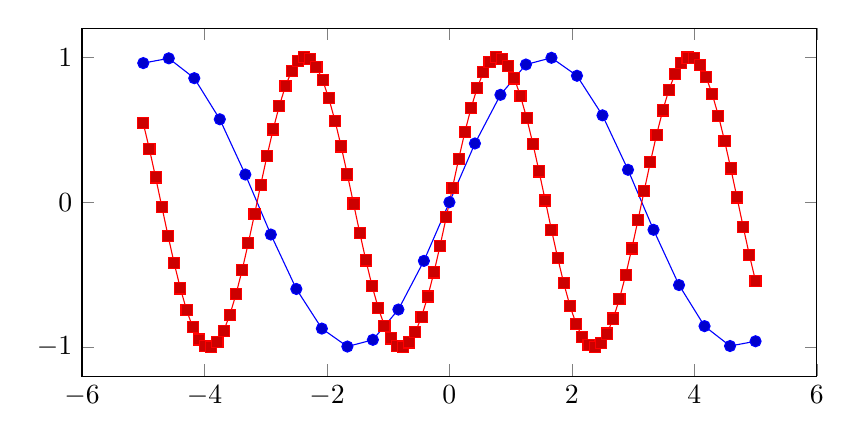
\begin{tikzpicture}
				\begin{axis}[
					width=0.9\textwidth,
					height=6cm,
					]
					
					\addplot {sin(deg(x))};
					\addplot+[samples=100] {sin(deg(2*x))};
				
				\end{axis}
			\end{tikzpicture}
			\caption{A nice sinus plot with Tikz.}
		\end{figure}
	\end{frame}
	
	% FRAME
	\begin{frame}{Bar charts}
		\begin{figure}
			\centering
			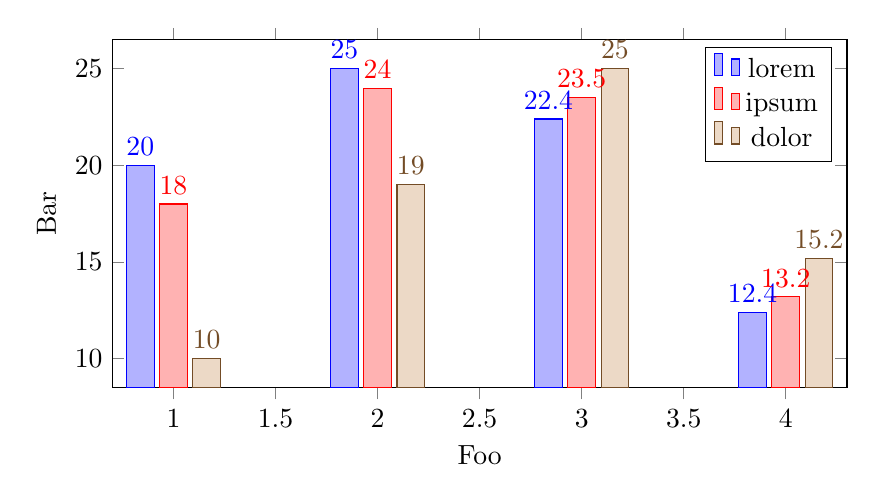
\begin{tikzpicture}
				\begin{axis}[
						ybar,
						xlabel={Foo},
					  	ylabel={Bar},
					  	width=0.9\textwidth,
					  	height=6cm,
						nodes near coords,
						nodes near coords align={vertical},
					]
					
					\addplot plot coordinates {(1, 20) (2, 25) (3, 22.4) (4, 12.4)};
					\addplot plot coordinates {(1, 18) (2, 24) (3, 23.5) (4, 13.2)};
					\addplot plot coordinates {(1, 10) (2, 19) (3, 25) (4, 15.2)};
					
					\legend{lorem, ipsum, dolor}
				
				\end{axis}
			\end{tikzpicture}
			\caption{A nice bar chart with Tikz.}
		\end{figure}
	\end{frame}
	
	% FRAME
	\begin{frame}{Quotes}
		\begin{quote}
			Veni, Vidi, Vici
		\end{quote}
		from Julius Caesar.
	\end{frame}
		
	% FRAME
	\begin{frame}[fragile]{References}
		Some references to showcase \verb|[allowframebreaks]| on next slide~\cite{Knuth92,ConcreteMath,Simpson,Er01,greenwade93}
	\end{frame}

	% % FRAME
	% \begin{frame}{References}
	% 	\bibliography{pres}
	% 	\bibliographystyle{abbrv}
	% \end{frame}

	% FRAME
	\begin{frame}[allowframebreaks]{References}
      \begin{thebibliography}{1}

         \bibitem{Er01}
         P.~Erd{\H o}s.
         \newblock A selection of problems and results in combinatorics.
         \newblock In {\em Recent trends in combinatorics (Matrahaza, 1995)}, pages 1--6. Cambridge Univ. Press, Cambridge, 1995.
         
         \bibitem{ConcreteMath}
         R.~Graham, D.~Knuth, and O.~Patashnik.
         \newblock {\em Concrete mathematics}.
         \newblock Addison-Wesley, Reading, MA, 1989.
         
         \bibitem{greenwade93}
         G.~D. Greenwade.
         \newblock The {C}omprehensive {T}ex {A}rchive {N}etwork ({CTAN}).
         \newblock {\em TUGBoat}, 14(3):342--351, 1993.
         
         \bibitem{Knuth92}
         D.~Knuth.
         \newblock Two notes on notation.
         \newblock {\em Amer. Math. Monthly}, 99:403--422, 1992.
         
         \bibitem{Simpson}
         H.~Simpson.
         \newblock Proof of the {R}iemann {H}ypothesis.
         \newblock preprint (2003), available at \texttt{http://www.math.drofnats.edu/riemann.ps}, 2003.
         
      \end{thebibliography}
   \end{frame}
	
\end{document}



% \documentclass[aspectratio=169]{beamer}
\usetheme{gotham}

	\usepackage{standalone}
	\usepackage{tikz}
	\usepackage{pgfplots}
	\usepackage{tabularray} % Typeset tabulars and arrays (contains equivalent of longtable, booktabs and dcolumn at least)
		\UseTblrLibrary{booktabs} % to load extra commands from booktabs
	\usepackage{changepage}
	\usepackage{minted}
		\definecolor{codeback}{rgb}{0.90,0.91,0.92}
		\definecolor{codebackdark}{rgb}{0.10,0.11,0.12}

	\newcommand{\famName}[1]{\textsc{#1}}
	\newcommand{\themename}{\textbf{\textsc{Gotham}}}


\begin{document}

\section{Gotham Theme}

	% FRAME
	\begin{frame}[fragile]{Gotham package}

		The \themename{} theme is a Beamer theme with a minimal-ish visual style largely inspired by the \href{https://github.com/matze/mtheme}{\textsc{Metropolis} Beamer Theme} by Matthias \famName{Vogelgesang} (and some other Beamer themes).

		Yet, \themename{} is highly extendable and versatile.
		\bigskip

		First, enable the theme by classically loading it:

		\begin{minted}{tex}
			\documentclass{beamer}
			\usetheme{gotham}
		\end{minted}

		Then, all the customization can be performed at any moment in the presentation using:

		\begin{minted}{tex}
			\gothamset{<option>=...}
		\end{minted}
	\end{frame}


\subsection{Fonts}

	% FRAME
	\begin{frame}[fragile]{Gotham title formats}
		Note, that you have to have Mozilla's \emph{Fira Sans} font and XeTeX or LuaTeX installed to enjoy this wonderful typography.

		\begin{columns}[T,onlytextwidth]
		\column{0.49\textwidth}
			\themename{} supports 4 different title formats \mintinline{tex}|\gothamset{format frametitle=}|
			\begin{itemize}
				\item regular
				\item \MakeLowercase{Lower}
				\item \MakeUppercase{Upper}
				\item \MakeTitlecase{Title Case}
			\end{itemize}
		\column{0.49\textwidth}
			\themename{} supports 3 different title shape \mintinline{tex}|\gothamset{shape frametitle=...}|:
			\begin{itemize}
				\item regular
				\item \textsc{Small caps}
				\item \textit{italic}
			\end{itemize}
		\end{columns}

		\vspace{2em}
		They can either be set at once for every title type or individually.
	\end{frame}

	{ \gothamset{format frametitle=upper, shape frametitle=italic}
	% FRAME
	\begin{frame}{Titles: Upper and italic}
		This frame uses the title format options: \mintinline{tex}|format frametitle=upper|, \mintinline{tex}|shape frametitle=italic|.
	\end{frame}
	}

	{ \gothamset{shape frametitle=smallcaps, format frametitle=titlecase}
	% FRAME
	\begin{frame}{Titles: Small caps and titlecase}
		This frame uses the title format options: \mintinline{tex}|shape frametitle=smallcaps|, \mintinline{tex}|format frametitle=titlecase|.
		
		\begin{alertblock}{Potential Problems}
			Be aware that not every font supports small caps.
			If for example you typeset your presentation with pdfTeX and the Computer Modern Sans Serif font, every text in \mintinline{tex}{smallcaps} will be typeset with the Computer Modern Serif font instead.
			Please refer to the documentation if you consider using it.
			
			As a rule of thumb: just use it for plaintext-only titles.
		\end{alertblock}
	\end{frame}
	}

	{ \gothamset{format frametitle=lower}
	% FRAME
	\begin{frame}{Titles: LOWER and regular}
		This frame uses the title format options: \mintinline{tex}{format frametitle=lower}, \mintinline{tex}{shape frametitle=regular}.
	\end{frame}
	}


\subsection{Colors}

	{ \gothamset{background=dark}
	% FRAME
	\begin{frame}[fragile]{Presentation style via background color}
		The color mode (a.k.a. background color) can be changed using:
		\begin{minted}[bgcolor=codebackdark]{tex}
			\gothamset{background=dark | light | transparent}
		\end{minted}
	\end{frame}
	}

	% FRAME
	\begin{frame}[fragile]{Blocks}
		Three different block environments are pre-defined and may be styled with an optional background color.

		\begin{columns}[T,onlytextwidth]
		\column{0.3\textwidth}
			\begin{minted}{tex}
				\gothamset{
					block=native}
			\end{minted}

			\gothamset{block=native}
			\begin{block}{Default}
				Block content.
			\end{block}

			\begin{alertblock}{Alert}
				Block content.
			\end{alertblock}

			\begin{exampleblock}{Example}
				Block content.
			\end{exampleblock}

		\column{0.3\textwidth}

			\gothamset{block=transparent}
			\begin{minted}{tex}
				\gothamset{
					block=transparent}
			\end{minted}

			\begin{block}{Default}
				Block content.
			\end{block}

			\begin{alertblock}{Alert}
				Block content.
			\end{alertblock}

			\begin{exampleblock}{Example}
				Block content.
			\end{exampleblock}

		\column{0.3\textwidth}

			\gothamset{block=fill}
			\begin{minted}{tex}
				\gothamset{
					block=fill}
			\end{minted}

			\begin{block}{Default}
				Block content.
			\end{block}

			\begin{alertblock}{Alert}
				Block content.
			\end{alertblock}

			\begin{exampleblock}{Example}
				Block content.
			\end{exampleblock}

		\end{columns}
	\end{frame}

	{\gothamset{colorset=red}
	% FRAME
	\begin{frame}[fragile]{Color customization}
		The color theme can be used only in preamble with \mintinline{tex}|\usecolortheme{wolverine}| and without guarantees on the visual aspect.

		\themename{} offers predefined color setup at any time through \mintinline{tex}|\gothamset{colorset=red}|

		Otherwise, the colors can be changed manually using:
		\begin{minted}{tex}
			\colorlet{colorPale}{gPaleYell} % BG in light/normal mode
			\colorlet{colorDark}{gDarkBlack} % FG in light/normal mode
			\colorlet{colorA}{gDarkTeal} % frametitle, standin.out,
			\colorlet{colorAreversed}{gLightTeal} % frametitle, standin.in,
			\colorlet{colorB}{gMidGrey} % gray BG : progress bar, blocks
			\colorlet{colorC}{gDeepYellOr} % progress bar
			\colorlet{colorD}{gLightOrange} % alert
			\colorlet{colorE}{gLightGreen} % example
		\end{minted}
	\end{frame}
	}


\subsection{Inner}

	% FRAME
	\begin{frame}[fragile]{Title page}
		\themename{} offers the possibility to adapt the title page layout (printed with \mintinline{tex}|\maketitle| or \mintinline{tex}|\titlepage|).
		This can be achieved using:
		\begin{minted}{tex}
			\defbeamertemplate{title page}{your name}{your defintion}
			\gothamset{title page= your name}
		\end{minted}

		\themename{} also predefined several templates such as:
		\mintinline{tex}$gotham normal$ | \mintinline{tex}$gotham splitvert$ | \mintinline{tex}$gotham dividedpic$ | \mintinline{tex}$gotham reversed$
	\end{frame}

	% FRAME
	\begin{frame}[fragile]{Table of contents}
		\themename{} comes with the possibility to apply different styles for your table of contents (ToC) page.
		You can define your own ToC style as it follows:
		\begin{minted}{tex}
			\defbeamertemplate{toc page}{your name}{your def}
			\gothamset{tocframe template= your name}
		\end{minted}
		Then, referring to this template using the frame option \mintinline{tex}|[toc]| in your presentation:
		\begin{minted}{tex}
			\begin{frame}[toc]{Table of contents}
				\tableofcontents%[hideallsubsections]
			\end{frame }
		\end{minted}

		Or using one of the \themename{} predefined templates, such as: \mintinline{tex}$gotham simple | gotham bullet$
	\end{frame}

	% FRAME
	\begin{frame}[fragile]{Sections}
		\themename{} provides a multiple options to tune sections (respectively \mintinline{tex}|part|, \mintinline{tex}|section|, \mintinline{tex}|subsection| and \mintinline{tex}|subsubsection|).

		The section command \mintinline{tex}|\section{Elements}| from Beamer will appear very different.
		The section page will appear or disappear thanks to: \mintinline{tex}$\gothamset{sectionframe default=<on|off>}$, while its layout (when appearing) is controlled by:
		\begin{minted}{tex}
			\defbeamertemplate{part|sub|subsub|section frame}
				{your name}{your def}
			\gothamset{sectionframe template= your name}
		\end{minted}

		\themename{} predefined template are: \mintinline{tex}$gotham progressbar | gotham simple |$ \mintinline{tex}$gotham splitvert progressbar |$ \mintinline{tex}$gotham splitvert simple | gotham progressvert$
	\end{frame}

	% FRAME
	\begin{frame}[fragile]{Sections contents}
		After the section page, you can (de)activate a page with a table of contents for the section using \mintinline{tex}$\gothamset{sectiontocframe default=<on|off>}$, and its layout is controlled by:
		\begin{minted}{tex}
			\defbeamertemplate{toc subsection frame}{your name}{your def}
			\gothamset{sectionframe template= your name}
		\end{minted}

		\themename{} predefined template are: \mintinline{tex}$gotham simple | gotham bullet$
	\end{frame}

	% FRAME
	\begin{frame}[fragile, watermark]{Watermark}

		With \themename{} you can locally or globally add watermark to your slides by using:
		\begin{minted}{tex}
			\defbeamertemplate{background}{watermark/your name}{your def}
			\gothamset{watermark template= your name}
		\end{minted}

		Then, this watermark can be turned on locally using \mintinline{tex}|\begin{frame}[watermark]| or globally with \mintinline{tex}|\gothamset{watermark default= on}| .
	\end{frame}

	% FRAME
	\begin{standinenv}
	\begin{frame}[fragile]{Standin}

		\themename{} comes with 2 environments/special layouts named \mintinline{tex}|standin| and \mintinline{tex}|standout|.
		These special layouts can be used to emphasize some content or last slide\textellipsis

		This layout can be turned on using \mintinline{tex}|\begin{frame}[standin]| or using the dedicated environment (\mintinline{tex}|\begin{standinenv}\begin{frame}...\end{frame}\end{standinenv}|).

		Note that the background can also be tuned using:
		\begin{minted}{tex}
			\defbeamertemplate{background canvas}{standin/name}{your def}
			\gothamset{standin BG template= name}
		\end{minted}

	\end{frame}
	\end{standinenv}

	% FRAME
	\begin{frame}[standout, watermark]{Standout}
		Here is an example of standout (working as standin), which can be combined with a watermark.

		Another difference, apart the obvious color change is the font size and series.
	\end{frame}


\subsection{Outer}

	{\setbeamertemplate{frame footer}{My custom footer}
	% FRAME
	\begin{frame}[fragile]{Frame footer}
		\themename{} defines a custom Beamer template to add a text to the footer.
		It can be set via
		\begin{minted}{tex}
			\setbeamertemplate{frame footer}{My custom footer}
		\end{minted}

		Even after redefining (or not) your frame footer template, you can locally remove it with the frame option \mintinline{tex}|\begin{frame}[nofooter]|.
	\end{frame}
	}

	\title[your shorttitle]{Gotham}
	\date[shortdate]{\today}
	\author[your shortauthor name]{Romain NOËL}
	% FRAME
	\begin{frame}[fragile, rotateFooter]{rotateFooter}
		The default footer from \themename{}, it displays the \mintinline{tex}|shortdate|, \mintinline{tex}|shorttitle| and \mintinline{tex}|shortauthor|.
		So by filling these fields in your document setup, you will see them appear in your footer:
		\begin{minted}{tex}
			\title[your shorttitle]{Your title}
			\date[shortdate]{\today}
			\author[your shortauthor name]{John DOE}
		\end{minted}

		Since we always need some extra space on some frames that would like to overlay a bit the footer, \themename{}'s footer also offers possibility to be put locally on the side using \mintinline{tex}|\begin{frame}[rotateFooter]|, or globally with
		\begin{minted}{tex}
			\gothamset{rotateFooter default=on}
		\end{minted}
		If it has set globally, it can be deactivated locally with the frame option \mintinline{tex}|\begin{frame}[norotateFooter]|.
	\end{frame}

	\title[]{Gotham}
	\date[]{\today}
	\renewcommand{\gothamRightFiligrane}{%
		\rotatebox{90}{gotham right filigrane pattern}
	}
	% FRAME
	\begin{frame}[edging, fragile]{Edging}
		\themename{} has two hook commands, \mintinline{tex}|\gothamRightFiligrane| and \mintinline{tex}|\gothamLeftFiligrane|, that can be redefined to customize what to display in the edgings (a.k.a. filigrane, a.k.a. sidebar).
		As an example, one could do:
		\begin{minted}{tex}
			\renewcommand{\gothamRightFiligrane}{%
				\rotatebox{90}{gotham right filigrane pattern}
			}
		\end{minted}

		Then, to set if it should be displayed or not, globally
		\begin{minted}{tex}
			\gothamset{edging default=on}
		\end{minted}
		or locally with the frame option \mintinline{tex}|\begin{frame}[edging]| or \mintinline{tex}|\begin{frame}[noedging]|.
	\end{frame}

	% FRAME
	% \begin{nofootlineenv}
	\begin{frame}[fragile,noedging,nofooter]{Really wide contents}
		\begin{adjustwidth}{-2em}{-2em}
			If you want a really wide content in your frame, you can change the size of your margin (requires \mintinline{tex}|\usepackage{changepage}| in your preamble).
			You can also suppress the edging (\mintinline{tex}|[noedging]|) and footer (\mintinline{tex}|[nofooter]|) or even more radically footline (\mintinline{tex}|[nofootline]|).

			Here is an example combining them:
			\begin{minted}{tex}
				\begin{frame}[noedging,nofootline]{extended frame}
					\begin{adjustwidth}{-2em}{-2em}% 2em extra to the left and 2em for right margin.
						wide content
					\end{adjustwidth}
				\end{frame }
			\end{minted}
		\end{adjustwidth}
	\end{frame}
	% \end{nofootlineenv}

	{%
	\renewcommand{\gothamInstituteLogoSquare}[1][4ex]{%
		
\includegraphics[height=#1]{gotham-logo.pdf}
	}
	\logo{extra LOGO}
	% FRAME
	\begin{frame}[fragile]{Frametitle}
		\framesubtitle{with a subtitle}
		The frametile template brought by \themename{} is relatively classic: it supports \mintinline{tex}|\subframetitle| and frame continuation (with \mintinline{tex}|[allowframebreaks]|) through templates that can be tuned.
		Nevertheless, it the frametitle template also includes a hook for your institute logo in the top right corner, leaving the command \mintinline{tex}|\logo{}| free for your extra logos.

		So, one can have both logos using:
		\begin{minted}{tex}
			\renewcommand{\gothamInstituteLogoSquare}[1][4ex]{
				
\includegraphics[height=#1]{gotham-logo.pdf}
			}
			\logo{extra LOGO}
		\end{minted}
	\end{frame}
	}

	\author[]{Romain NOËL}
	{\gothamset{progressbar position=left, progressbar style= rounded box, progressbar advancement= brlt,  numbering= circle}
	% FRAME
	\begin{frame}[fragile]{Numbering and progressbar}

		\themename{} theme can numbering your frames in the bottom right corner using different styles.
		You can also decide to use a progression bar to indicate how much of your presentation remains.

		The setup of numbering and progression bar can be performed through:
		\begin{minted}{tex}
			\gothamset{numbering= totalframenumber, progressbar position=foot}
		\end{minted}

		Numbering available options are: \mintinline{tex}$none | framenumber | totalframenumber | appendixframenumber | pagenumber $ \mintinline{tex}$| totalpagenumber | circle$

		Progressbar position available options are: \mintinline{tex}$none | head | frametitle | foot | circlehead | left | right$
	\end{frame}
	}


\end{document}
%EoF


\documentclass[aspectratio=169]{beamer}
\usetheme{gotham}

   \usepackage{appendixnumberbeamer}
   \usepackage[scale=2]{ccicons}
   \newcommand{\themename}{\textbf{\textsc{Gotham}}}


\begin{document}

\section{Concluding Remarks}

	% FRAME
	\begin{frame}{Summary}
		Get the source of this theme and the demo presentation from

		\begin{center}\url{https://gitlab.com/RomainNOEL/beamertheme-gotham}\end{center}

		The theme \emph{itself} is licensed under a \href{http://creativecommons.org/licenses/by-sa/4.0/}{Creative Commons Attribution-ShareAlike 4.0 International License}.
		\begin{center} \ccbysa \end{center}
	\end{frame}

	% FRAME
   \begin{standoutenv}
   \begin{frame}[fragile]
      The final slide using the standout style with command:
		\begin{verbatim}
			\begin{frame}[standout, plain]{Thank You !}
				Questions ?
		 	\end{frame }
		\end{verbatim}

		\begin{center}
			Et voilà !
		\end{center}
   \end{frame}
   \end{standoutenv}
	
\end{document}




\appendix

	\begin{frame}[fragile]{Backup slides}
		Sometimes, it is useful to add slides at the end of your presentation to refer to during audience questions.

		The best way to do this is to include \verb|\usepackage{appendixnumberbeamer}| in your preamble and call \verb|\appendix| before your backup slides.

		\themename{} will automatically turn off slide numbering and progress bars for slides in the appendix.
	\end{frame}


\end{document}
